\chapter{Hardware}
\label{Hardware}
\section{Überblick}

Vielleicht könnte dieses Schema hier viel gewinnbringender eingefügt werden als im Abschnitt Grobkonzept?

\begin{figure}[H]
	\centering
	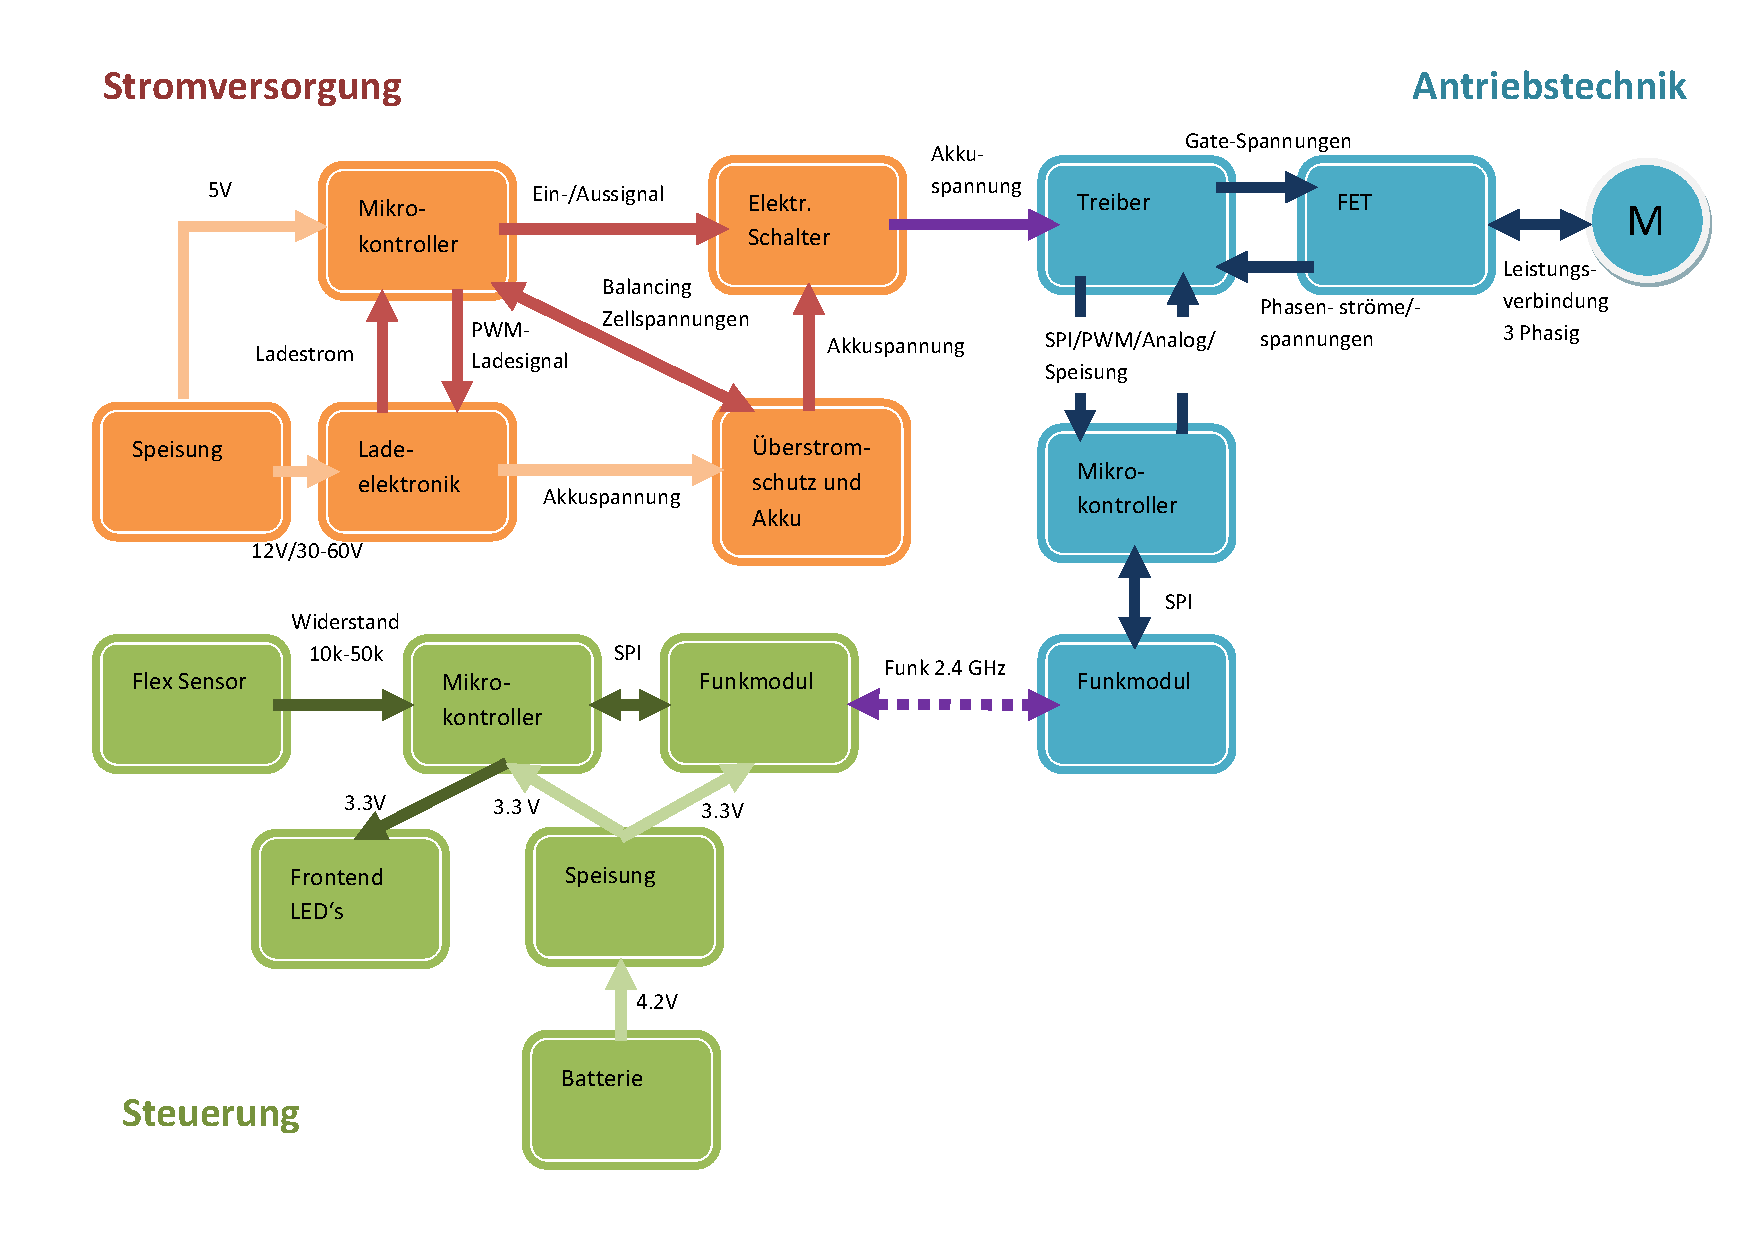
\includegraphics[width=1\linewidth]{images/Grobkonzept_Blockschaltbild_detailliert}
	\caption[Detailliertes Blockschaltbild]{Detailliertes Blockschaltbild}
	\label{fig:grobkonzeptblockschaltbilddetailliert_2}
\end{figure}


\section{Steuerung - Magic-Glove}
\label{HW_MagicGlove}

\section{Stromversorgung}
\label{HW_Stromversorgung}
Die Stromversorgung ist für dafür Zuständig, das der Akku fachgerecht geladen wird. Zusätzlich überwacht die Schaltung, das der Akku weder überladen, noch tiefentladen wird.
\subsection*{Balancing}

\subsection*{Ladeelektronik}
\subsection*{Mikrocontroller}


\section{Motoransteuerung}
\label{HW_Motoransteuerung}
\subsection*{Treiber IC und Speisung}
\subsection*{Endstufe (H-Brücke)}
\subsection*{Messschaltung}
\subsection*{Mikrocontroller}

